\section{Conclusion}
\subsection{Objectives completition}
It can be said that the proyect \textit{Design, construction and programming of a low cost, Open Source robot for assistive activities} has accomplished the objectives originally set:

	\begin{itemize}

	\item Different configurations have been studied in order to achieve a working prototype

	\item The final design, derived from the previous study has been modelled using the CAD program SketchUp

	\item The modelled parts have been created by means of a 3D printer

	\item The parts have been assembled and the electronics installed in order to create a functioning robot

	\item The Arduino board has been programmed to control both the arms as the base following the user's commands

	\item The Raspberry Pi has been programmed to:

		\begin{itemize}
		
		\item set up a wifi network that enables bidirectional communication between the user and the PD-SD independently of pre-existing networks

		\item stream the video feed captured by the on-board camera to the user's phone

		\item receive the user's instructions and send them to the Arduino over serial communication while the socket connection maintained

		\item initialize a script when booting to do all the previous automatically

		\end{itemize}

	\item Program the Android application \textit{Bot Control} to allow the user to take control of the Droid while being able to monitor what it sees


	\end{itemize}



The robot is also low cost, as it can be seen in the ``Budget" annex and Open Source, as all of the code can be downloaded from this \href{https://github.com/alvaroferran/Proyecto}{GitHub repository} \footnote{https://github.com/alvaroferran/Proyecto}.\\

Finally, while it is a working prototype, it can be improved by implementing the suggestions found in the following section.





















\newpage
\subsection{Future work}

The PD-SD is a very versatile robot, but it is far from complete and many new features can be added. A few of them could be:

\paragraph{iOS application:} Although Android has the largest market share, iOS users are not negligeable, and the most immediate improvement would be to develop a version of Bot Control for that system, in order to increase the number potential users.

\paragraph{User routine programming:} Another interesting feature would be to include the ability for the non-technical user to program chores they want the robot to accomplish, such as bringing them a glass of water every morning or opening the blinds at a set hour. \\

This would give the users a higher quality service from their PD-SD, since they would be able to demand tasks as needed.



\paragraph{Enhanced gripper:}  The PD-SD currently features two parallel grippers, which enable it to grasp objects of different sizes due to the closing mechanism. However, complex figures may not be easy to hold to, and a vacuum gripper would be the ideal solution for this. By being pushed into the object while filled with air, the gripper adapts its shape to fit the object better, and when the air is removed the object remains firmly in place until it is released again. Figure \ref{gripper} illustrates this procedure.

	\begin{figure}[H]
			\centering
			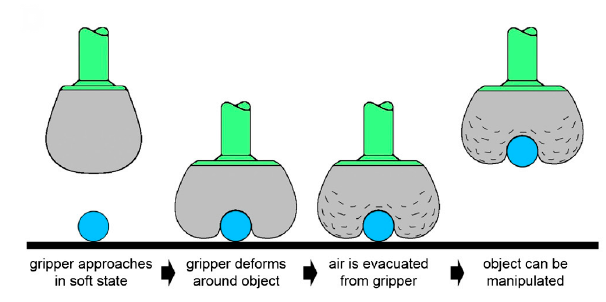
\includegraphics[scale=0.7]{images/Conclusion/gripper.png}
			\caption{Vacuum gripper  }
			\label{gripper}
	\end{figure}
	\bigskip


\paragraph{Full-size droid:} The final objective of this project is to eventually build a full-size robot capable of actually helping in the house by being able, for example, to reach into the higher cabinets of the kitchen or carry objects from one place to another.\\ 

In order to do this the robot must have a certain height and strength, so while the software would largely remain unchanged, the actuators and body parts would certainly need a revision. 


\paragraph{Computer vision:} Finally, adding computer vision capabilities to the robot would greatly enhance its capabilities. By integrating a library such as OpenCV, the robot could be able to recognize its charging dock by means of a symbol, or simply the phrase ``Charging dock", and could move towards it when the battery level descended.\\

Another feature would be to implement a pathfinding algorithim to take into account the walls, doors and floor of the house and make the robot navigate throughout it autonomously, for instance to fulfill one of the previously mentioned ``programmed chores".
